\documentclass{article}
\usepackage{fancyhdr}
\usepackage{ctex}
\usepackage{listings}
\usepackage{graphicx}
\usepackage[a4paper, body={18cm,22cm}]{geometry}
\usepackage{amsmath,amssymb,amstext,wasysym,enumerate,graphicx}
\usepackage{float,abstract,booktabs,indentfirst,amsmath}
\usepackage{array}
\usepackage{booktabs}
\usepackage{multirow}
\usepackage{url}
\usepackage{diagbox}
\usepackage{hyperref}
\usepackage{listings}
\renewcommand\arraystretch{1.4}
\usepackage{indentfirst}
\setlength{\parindent}{2em}
\usepackage{enumitem}
\usepackage{accsupp}
\setmonofont{Consolas}
\usepackage{listings}
\usepackage{xcolor}
\usepackage{makecell}
\usepackage{subfigure}
\usepackage{longtable}
\setCJKmonofont{黑体}
\newcommand\emptyaccsupp[1]{\BeginAccSupp{ActualText={}}#1\EndAccSupp{}}
\newcommand\SQL{\texttt{SQL}}
\renewcommand\tt{\texttt}
\lstset{
    % language = C,
    showstringspaces=false,
    xleftmargin = 3em,xrightmargin = 3em, aboveskip = 1em,
	backgroundcolor = \color{white}, % 背景色
	basicstyle = \small\ttfamily, % 基本样式 + 小号字体
	rulesepcolor= \color{gray}, % 代码块边框颜色
	breaklines = true, % 代码过长则换行
	numbers = left, % 行号在左侧显示
	numberstyle=\emptyaccsupp,
    numbersep = 14pt, 
    keywordstyle=\color{purple}\bfseries, % 关键字颜色
    commentstyle =\color{red!50!green!50!blue!60}, % 注释颜色
    stringstyle = \color{red}, % 字符串颜色
    morekeywords={ASSERT, int64_t, uint32_t},
	% frame = shadowbox, % 用(带影子效果)方框框住代码块
	frame = single, % 用(带影子效果)方框框住代码块
	showspaces = false, % 不显示空格
	columns = fixed, % 字间距固定
  framesep=1em
} 
\lstset{
    sensitive=true,
    moreemph={ASSERT, NULL}, emphstyle=\color{red}\bfseries,
    moreemph=[2]{int64_t, uint32_t, tid_t, uint8_t, int16_t, uint16_t, int32_t, size_t}, emphstyle=[2]\color{purple}\bfseries,
    showspaces = false, % 不显示空格
    }
%--------------------页眉--------------------%
\pagestyle{fancy}
\fancyhead[L]{}
\fancyhead[R]{}
\fancyhead[C]{《数据库系统及应用实践》课程实验报告}
\fancyfoot[C]{-\thepage-}
\renewcommand{\headrulewidth}{1.5pt}
%--------------------标题--------------------%
\begin{document}
\begin{center}
  \LARGE{{\textbf{\heiti 《数据库系统及应用实践》课程实验报告}}}

  \vspace{0.5em}

  \large 实验7:事务处理
  \begin{table}[H]
    \centering
    \begin{tabular}{p{2cm}p{2cm}<{\centering}p{0.4cm}p{2cm}p{3cm}<{\centering}p{0.4cm}p{2cm}p{3cm}<{\centering}}
      姓\qquad 名: & 李鹏达 & \quad & 学\qquad 号: & 10225101460 & \quad & 完成日期: & 2024年6月26日 \\ \cline{2-2} \cline{5-5} \cline{8-8}
    \end{tabular}
  \end{table}
\end{center}
% \rule{\textwidth}{1pt}
%--------------------正文--------------------%
\section{实验目标}
\begin{enumerate}[noitemsep]
  \item 学习和掌握MySQL数据库管理系统中事务处理相关的设置和基本操作;
  \item 学习和理解事务处理过程中不同事务隔离级别所对应的异常,能够根据应用场景选择合适的事务隔离级别;
\end{enumerate}

\section{实验过程记录}

在 Docker 容器中启动 MySQL 数据库。

\subsection{事务相关设置和基本操作}

启动三个 MySQL 客户端($T_1$, $T_2$, $T_3$),分别连接到数据库。

分别在不同客户端中执行下列语句,查看和修改系统变量的值;

\begin{lstlisting}[language=sql]
show global variables like 'autocommit'; -- T1
show session variables like 'autocommit'; -- T1
show global variables like '%transaction%'; -- T1
show session variables like '%transaction%'; --T1
set global autocommit = OFF; -- T1
set session autocommit = OFF; -- T1
select @@global.autocommit, @@session.autocommit; -- T1
select @@global.autocommit, @@session.autocommit; -- T2
\end{lstlisting}

结果如下:

\begin{figure}[H]
  \centering
  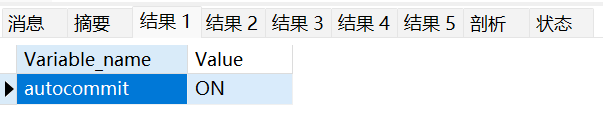
\includegraphics[width=0.3\textwidth]{img/1.png}
  \caption{T1执行结果(1)}
\end{figure}

\begin{figure}[H]
  \centering
  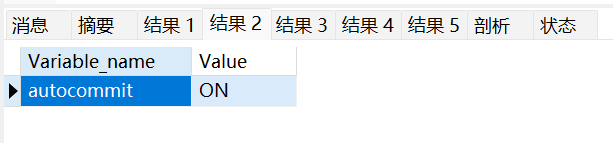
\includegraphics[width=0.3\textwidth]{img/2.png}
  \caption{T1执行结果(2)}
\end{figure}

\begin{figure}[H]
  \centering
  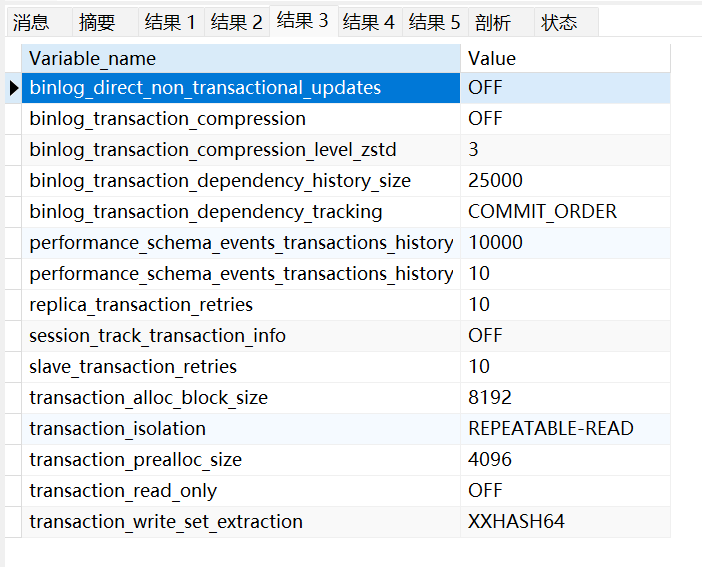
\includegraphics[width=0.6\textwidth]{img/3.png}
  \caption{T1执行结果(3)}
\end{figure}

\begin{figure}[H]
  \centering
  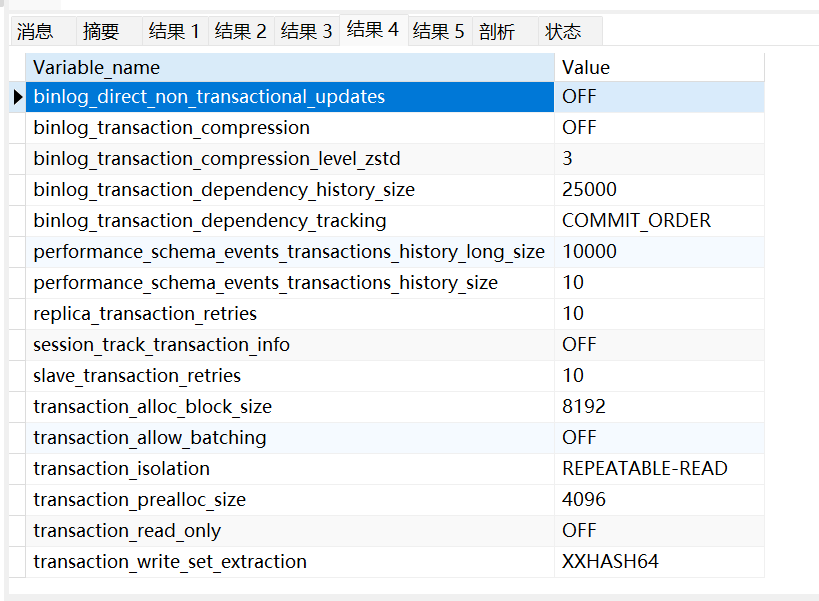
\includegraphics[width=0.6\textwidth]{img/4.png}
  \caption{T1执行结果(4)}
\end{figure}

\begin{figure}[H]
  \centering
  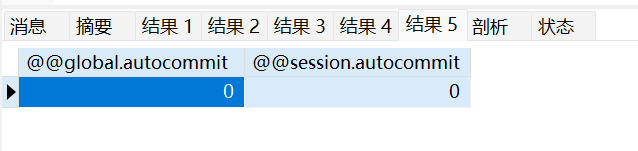
\includegraphics[width=0.6\textwidth]{img/5.png}
  \caption{T1执行结果(5)}
\end{figure}

\begin{figure}[H]
  \centering
  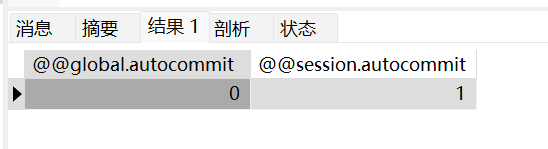
\includegraphics[width=0.6\textwidth]{img/6.png}
  \caption{T2执行结果}
\end{figure}

分别在不同客户端中执行下列语句,对比自动提交事务与手动提交事务的差别;

\begin{lstlisting}[language=sql]
insert into region values(5,'MOON','Inserted by a non-autocommit transaction.'); -- T1
insert into region values(6,'SUN','Inserted by an autocommit transaction.'); -- T2
start transaction; -- T3
insert into region values(7,'STAR','Inserted by a rollback transaction.'); -- T3
select * from region; -- T1
select * from region; -- T2
select * from region; -- T3
commit; -- T1
rollback; -- T3
select * from region; -- T1
select * from region; -- T2
select * from region; -- T3
\end{lstlisting}

结果如下:

\begin{figure}[H]
  \centering
  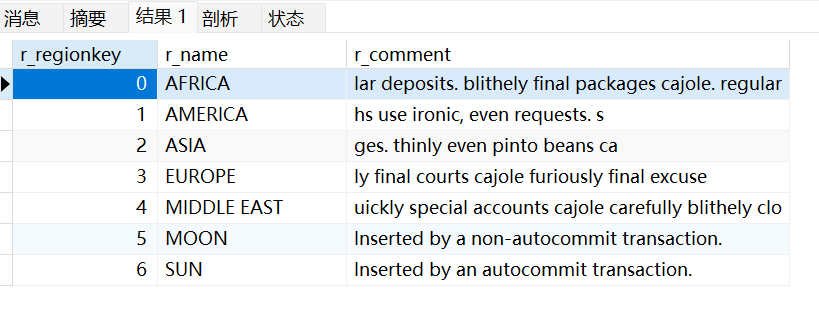
\includegraphics[width=0.6\textwidth]{img/7.png}
  \caption{T1执行结果(1)}
\end{figure}

\begin{figure}[H]
  \centering
  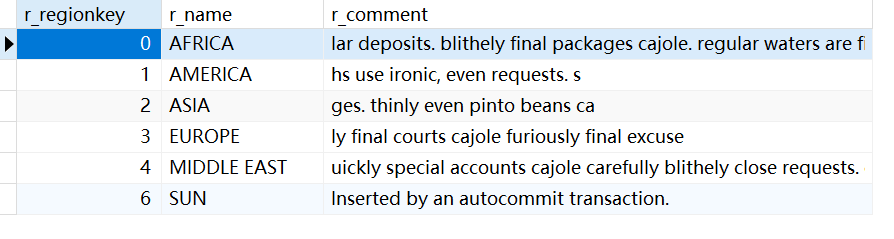
\includegraphics[width=0.6\textwidth]{img/8.png}
  \caption{T2执行结果(1)}
\end{figure}

\begin{figure}[H]
  \centering
  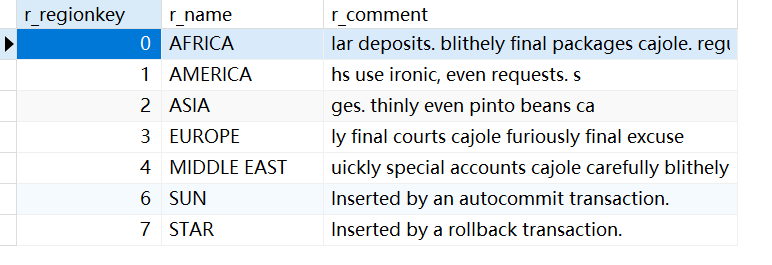
\includegraphics[width=0.6\textwidth]{img/9.png}
  \caption{T3执行结果(1)}
\end{figure}

\begin{figure}[H]
  \centering
  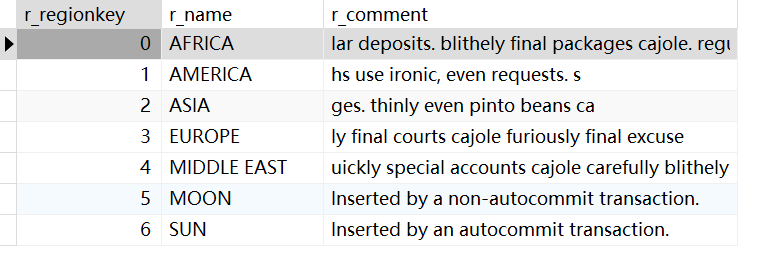
\includegraphics[width=0.6\textwidth]{img/10.png}
  \caption{T1执行结果(2)}
\end{figure}

\begin{figure}[H]
  \centering
  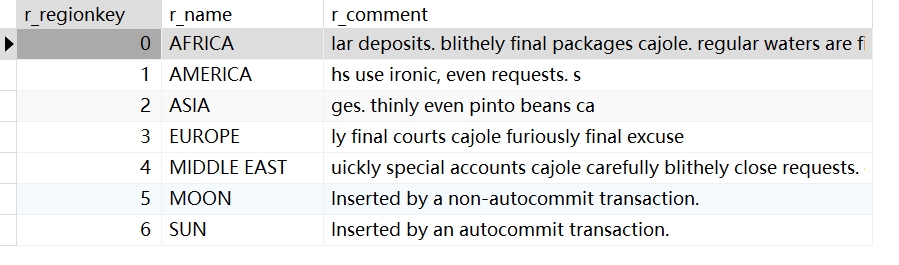
\includegraphics[width=0.6\textwidth]{img/11.png}
  \caption{T2执行结果(2)}
\end{figure}

\begin{figure}[H]
  \centering
  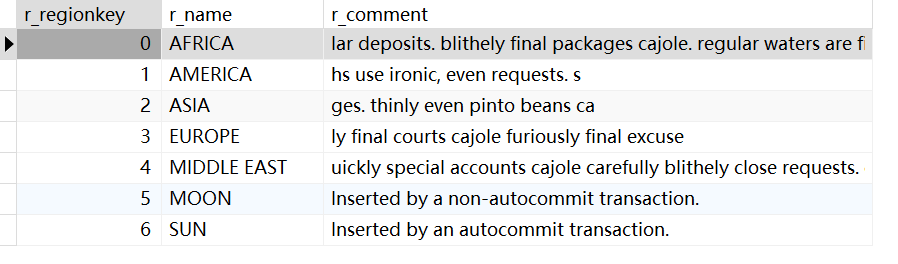
\includegraphics[width=0.6\textwidth]{img/12.png}
  \caption{T3执行结果(2)}
\end{figure}

分别在不同客户端中执行下列语句,关注不同语句对于事务的影响;

\begin{lstlisting}[language=sql]
start transaction; -- T2
delete from region where r_regionkey = 6; -- T2
select * from region; -- T1
select * from region; -- T2
select * from region; -- T3
rollback; -- T2
select * from region; -- T1
select * from region; -- T2
select * from region; -- T3
start transaction; -- T2
delete from region where r_regionkey = 6; -- T2
select * from region; -- T1
select * from region; -- T2
select * from region; -- T3
analyze table orders; -- T2
rollback; -- T2
select * from region; -- T1
select * from region; -- T2
select * from region; -- T3
commit; --T1
\end{lstlisting}

结果如下:

\begin{figure}[H]
  \centering
  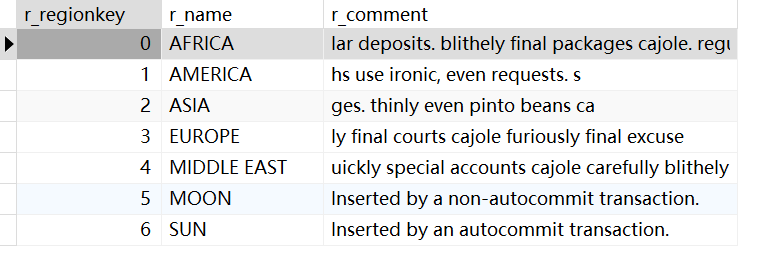
\includegraphics[width=0.6\textwidth]{img/13.png}
  \caption{T1执行结果(1)}
\end{figure}

\begin{figure}[H]
  \centering
  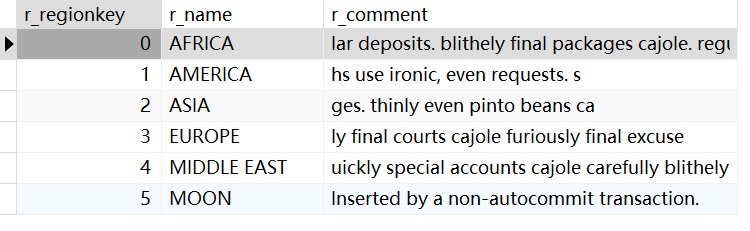
\includegraphics[width=0.6\textwidth]{img/14.png}
  \caption{T2执行结果(1)}
\end{figure}

\begin{figure}[H]
  \centering
  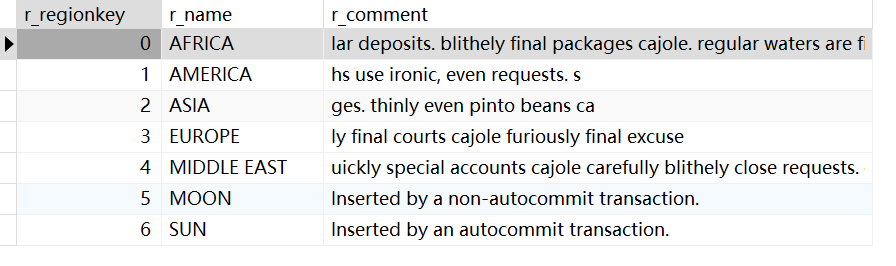
\includegraphics[width=0.6\textwidth]{img/15.png}
  \caption{T3执行结果(1)}
\end{figure}

\begin{figure}[H]
  \centering
  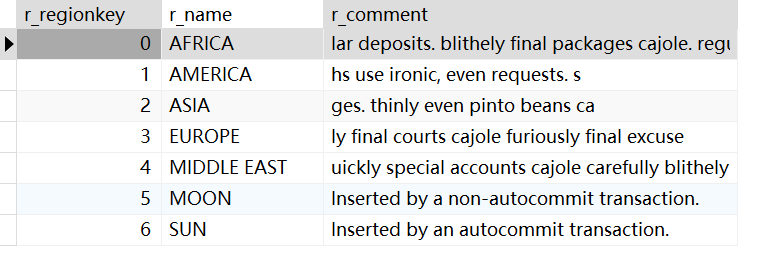
\includegraphics[width=0.6\textwidth]{img/16.png}
  \caption{T1执行结果(2)}
\end{figure}

\begin{figure}[H]
  \centering
  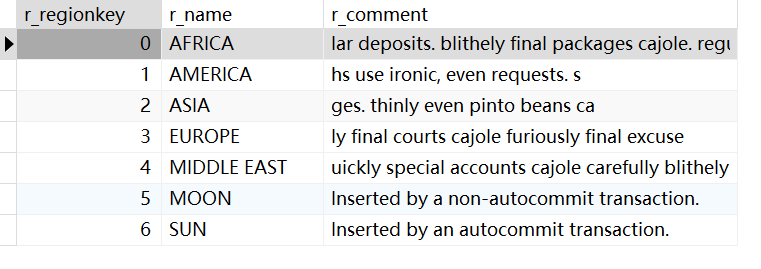
\includegraphics[width=0.6\textwidth]{img/17.png}
  \caption{T2执行结果(2)}
\end{figure}

\begin{figure}[H]
  \centering
  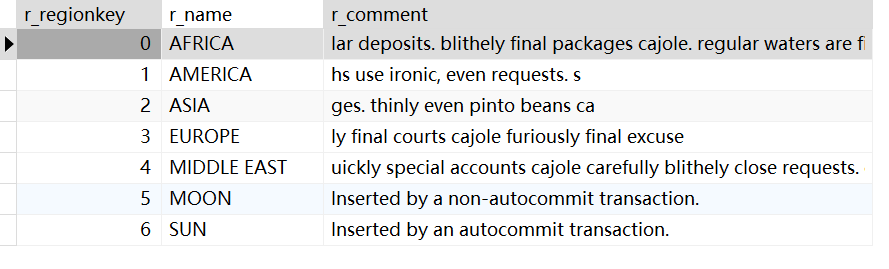
\includegraphics[width=0.6\textwidth]{img/18.png}
  \caption{T3执行结果(2)}
\end{figure}

\begin{figure}[H]
  \centering
  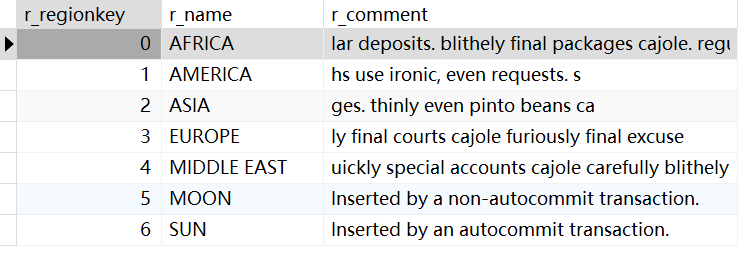
\includegraphics[width=0.6\textwidth]{img/19.png}
  \caption{T1执行结果(3)}
\end{figure}

\begin{figure}[H]
  \centering
  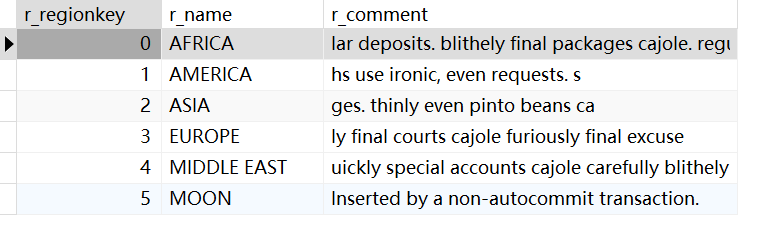
\includegraphics[width=0.6\textwidth]{img/20.png}
  \caption{T2执行结果(3)}
\end{figure}

\begin{figure}[H]
  \centering
  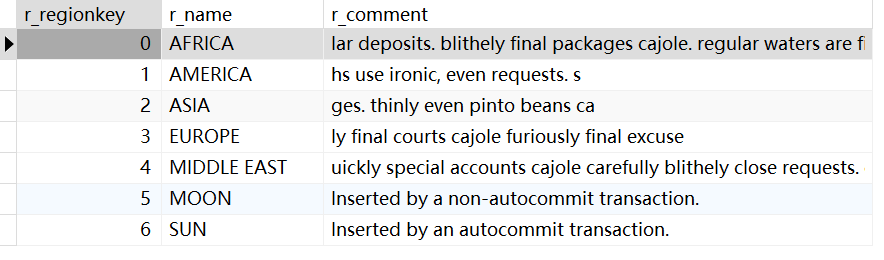
\includegraphics[width=0.6\textwidth]{img/21.png}
  \caption{T3执行结果(3)}
\end{figure}

\begin{figure}[H]
  \centering
  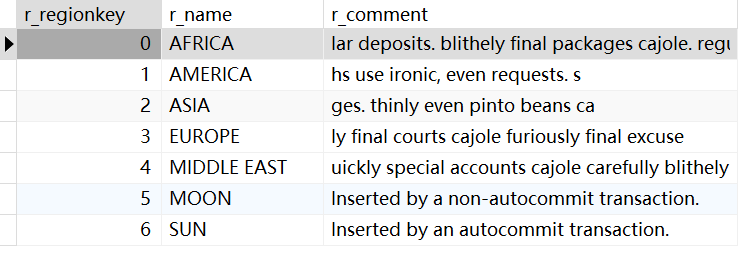
\includegraphics[width=0.6\textwidth]{img/22.png}
  \caption{T1执行结果(4)}
\end{figure}

\begin{figure}[H]
  \centering
  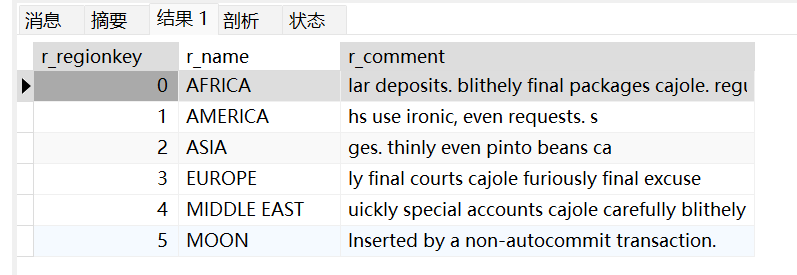
\includegraphics[width=0.6\textwidth]{img/23.png}
  \caption{T2执行结果(4)}
\end{figure}

\begin{figure}[H]
  \centering
  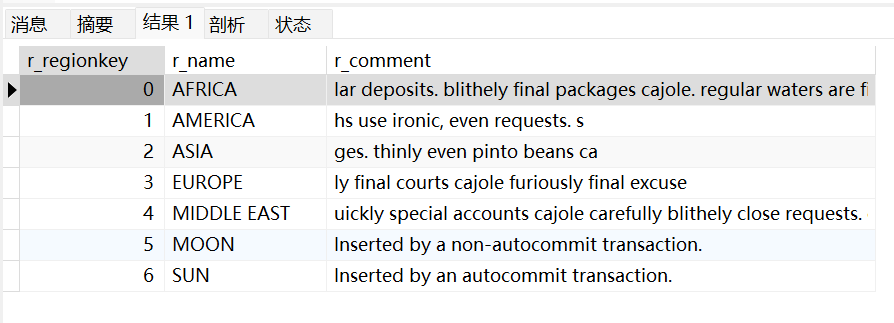
\includegraphics[width=0.6\textwidth]{img/24.png}
  \caption{T3执行结果(4)}
\end{figure}

在客户端T2中执行下列语句,关注如何使用SAVEPOINT;

\begin{lstlisting}[language=sql]
start transaction;
insert into region values(5,'MOON','Savepoint moon');
savepoint moon;
insert into region values(6,'SUN','Savepoint sun');
savepoint sun;
insert into region values(7,'STAR','Savepoint star');
savepoint star;
select * from region;
rollback to sun;
select * from region;
rollback to star;
select * from region;
rollback to moon;
select * from region;
commit;
\end{lstlisting}

结果如下:

\begin{figure}[H]
  \centering
  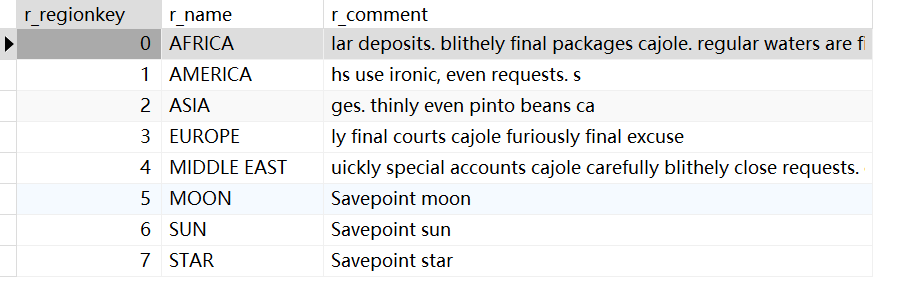
\includegraphics[width=0.6\textwidth]{img/25.png}
  \caption{T2执行结果(1)}
\end{figure}

\begin{figure}[H]
  \centering
  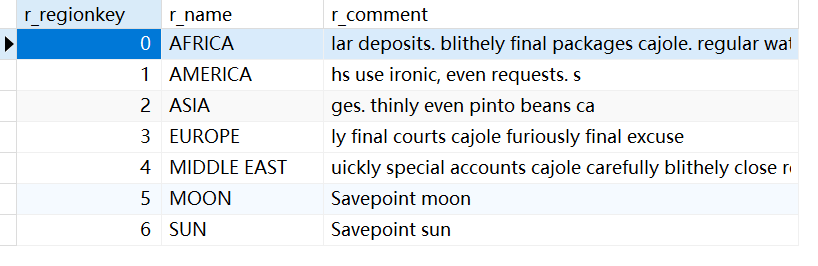
\includegraphics[width=0.6\textwidth]{img/26.png}
  \caption{T2执行结果(2)}
\end{figure}

\begin{figure}[H]
  \centering
  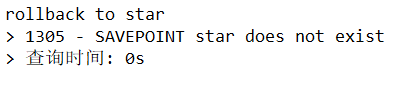
\includegraphics[width=0.6\textwidth]{img/27.png}
  \caption{T2执行结果(3)}
\end{figure}

\begin{figure}[H]
  \centering
  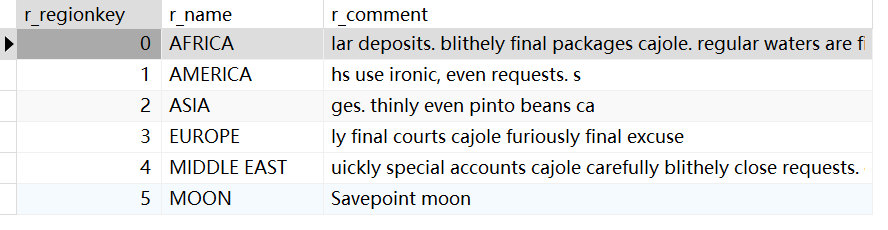
\includegraphics[width=0.6\textwidth]{img/28.png}
  \caption{T2执行结果(4)}
\end{figure}

可以发现,当回滚到 sun 后,就无法再回滚到 star 了,因为 star 是在 sun 之后创建的。

分别在不同客户端中执行下列语句,关注如何使用LOCK TABLES语句;

\begin{lstlisting}[language=sql]
lock tables region read; -- T2
select count(*) from region; -- T2
select count(*) from nation; -- T2
select * from region; -- T3
delete from region where r_regionkey = 5; -- T3
lock tables nation write, nation as n1 read; -- T2
insert into nation select n_nationkey+100, n_name, n_regionkey,n_comment
from nation; -- T2;
insert into nation select n_nationkey+100, n_name, n_regionkey,n_comment
from nation as n1; -- T2;
lock tables region read; -- T2
select * from region; -- T2
select * from region as r; -- T2
lock tables region as r read; -- T2
select * from region; -- T2
select * from region as r; -- T2
delete from nation where n_nationkey >= 100; -- T3
\end{lstlisting}

结果如下:

\begin{figure}[H]
  \centering
  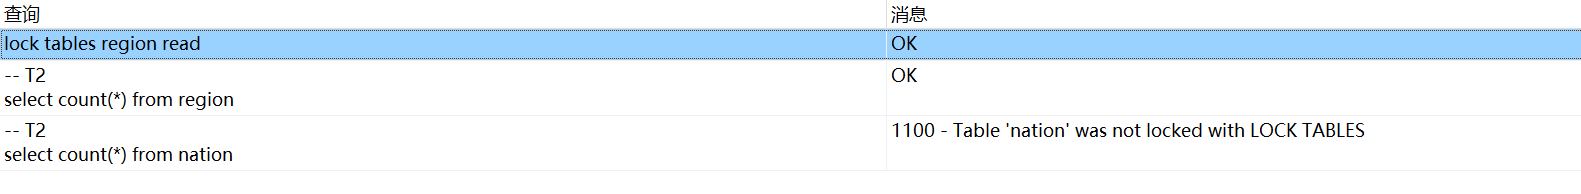
\includegraphics[width=0.9\textwidth]{img/29.png}
  \caption{T2执行结果(1)}
\end{figure}

可以发现,当 T2 给 region 表加锁后,T2 可以读取 region 表,但无法读取 nation 表。

\begin{figure}[H]
  \centering
  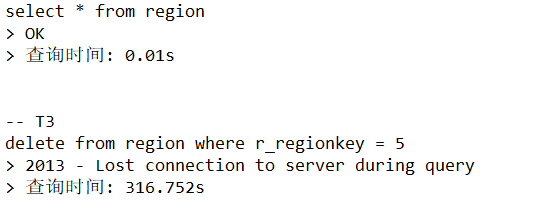
\includegraphics[width=0.9\textwidth]{img/30.png}
  \caption{T3 执行结果(1)}
\end{figure}

发现 T3 可以读取但无法删除 region 表中的数据,因为 region 表被 T2 锁住了。

\begin{figure}[H]
  \centering
  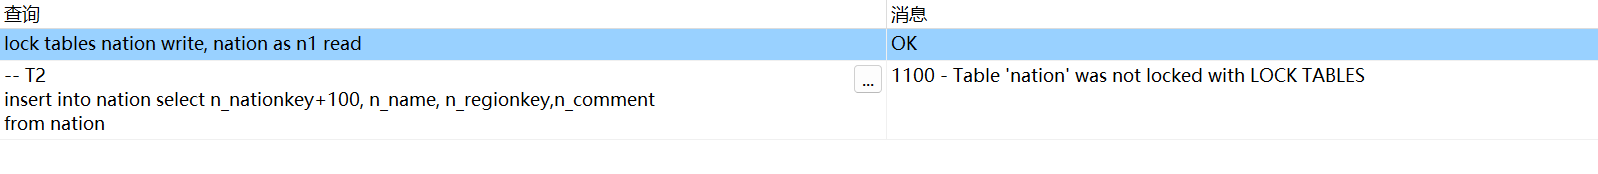
\includegraphics[width=0.9\textwidth]{img/31.png}
  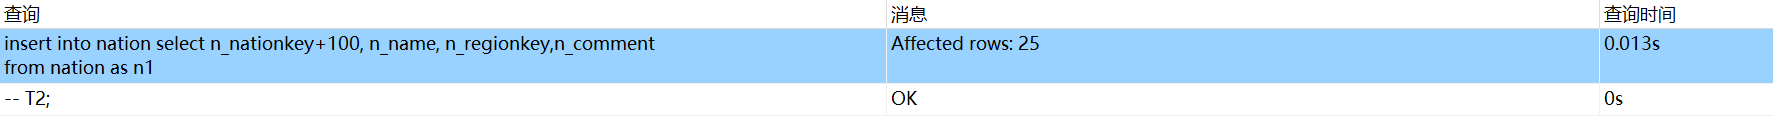
\includegraphics[width=0.9\textwidth]{img/32.png}
  \caption{T2 执行结果(2)}
\end{figure}

在获取 nation 表的写锁,和别名为 n1 的读锁后,在复杂查询中,必须使用别名来读取数据。

\begin{figure}[H]
  \centering
  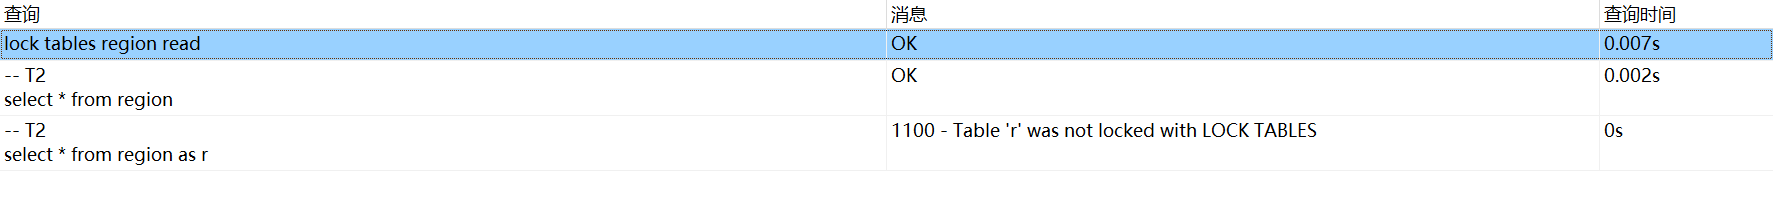
\includegraphics[width=0.9\textwidth]{img/33.png}
  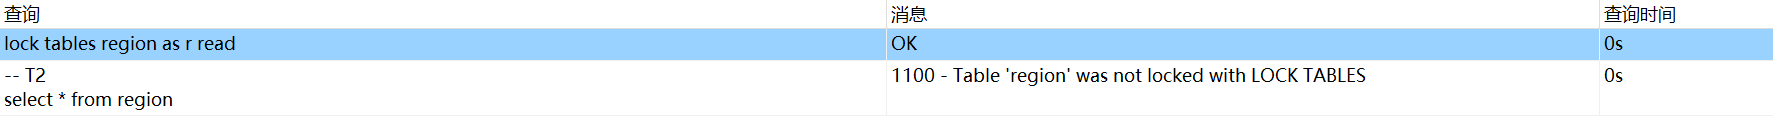
\includegraphics[width=0.9\textwidth]{img/34.png}
  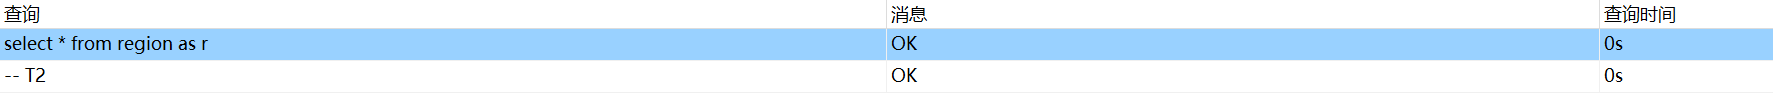
\includegraphics[width=0.9\textwidth]{img/35.png}
  \caption{T2 执行结果(3)}
\end{figure}

同时,获取锁时未使用别名,后续查询时则不能使用别名。使用别名获取锁后,后续查询也必须使用别名。

\begin{figure}[H]
  \centering
  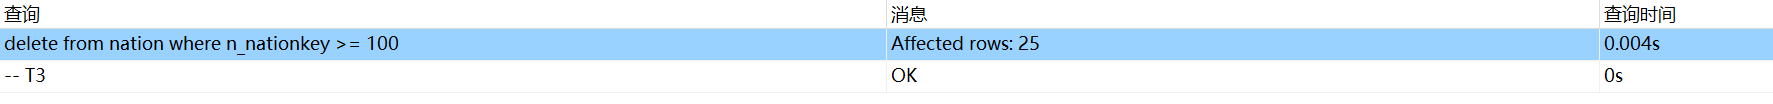
\includegraphics[width=0.9\textwidth]{img/36.png}
  \caption{T3 执行结果(2)}
\end{figure}

此时,T3 可以删除 nation 表中的数据。

在客户端T2中执行下列语句,关注如何设置事务属性;

\begin{lstlisting}[language=sql]
select @@global.transaction_isolation, @@global.transaction_read_only;
set global transaction isolation level serializable;
set global transaction read only;
select @@global.transaction_isolation, @@global.transaction_read_only;
select @@session.transaction_isolation, @@session.transaction_read_only;
set @@session.transaction_isolation = 'read-committed';
set @@session.transaction_read_only = on;
select @@session.transaction_isolation, @@session.transaction_read_only;
start transaction;
select * from region;
insert into region values(5,'MOON','Read only?');
set transaction_read_only = off;
insert into region values(5,'MOON','Read only?');
commit;
start transaction;
select * from region;
insert into region values(5,'MOON','Read only?');
rollback;
start transaction;
select @@global.transaction_isolation, @@session.transaction_isolation;
set transaction isolation level serializable;
select @@global.transaction_isolation, @@session.transaction_isolation;
set session transaction isolation level serializable;
select @@global.transaction_isolation, @@session.transaction_isolation;
commit;
\end{lstlisting}

结果如下:

\begin{figure}[H]
  \centering
  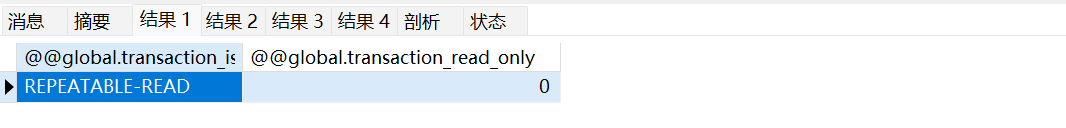
\includegraphics[width=0.9\textwidth]{img/37.png}
  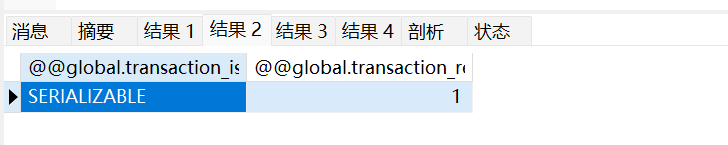
\includegraphics[width=0.9\textwidth]{img/38.png}
  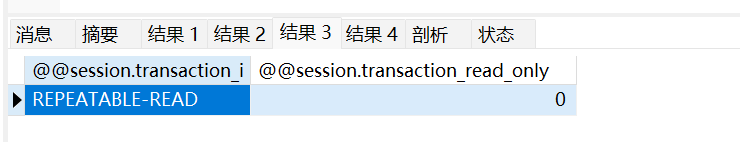
\includegraphics[width=0.9\textwidth]{img/39.png}
  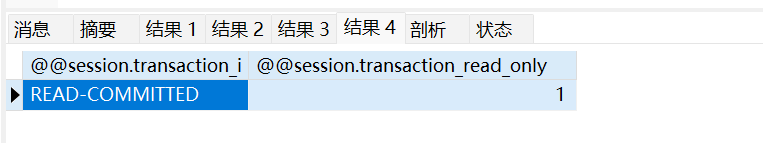
\includegraphics[width=0.9\textwidth]{img/40.png}
  \caption{T2 执行结果(1)}
\end{figure}

\begin{figure}[H]
  \centering
  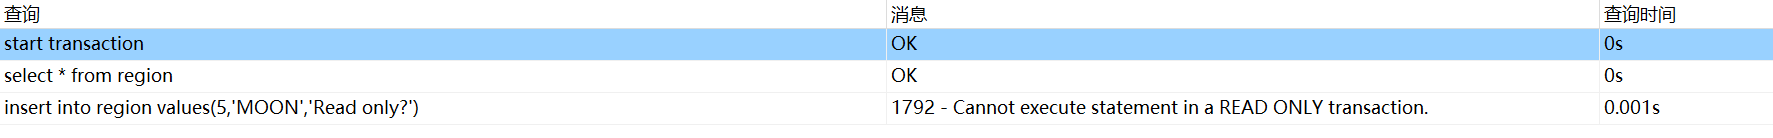
\includegraphics[width=0.9\textwidth]{img/41.png}
  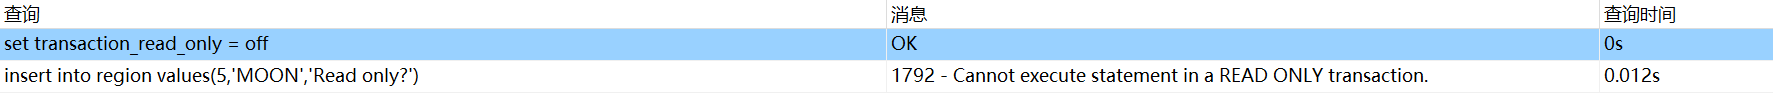
\includegraphics[width=0.9\textwidth]{img/42.png}
  \caption{T2 执行结果(2)}
\end{figure}

可以发现,在只读事务中,无法插入数据。

\begin{figure}[H]
  \centering
  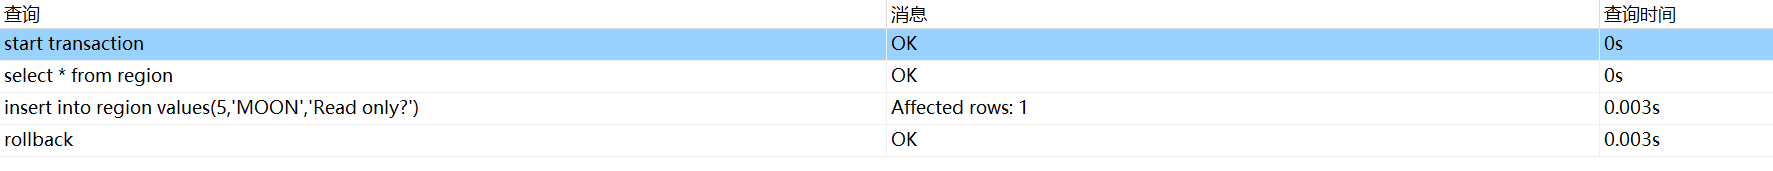
\includegraphics[width=0.9\textwidth]{img/43.png}
  \caption{T2 执行结果(3)}
\end{figure}

可以发现,只有当当前事务被提交后,对只读属性的修改才会生效。

\begin{figure}[H]
  \centering
  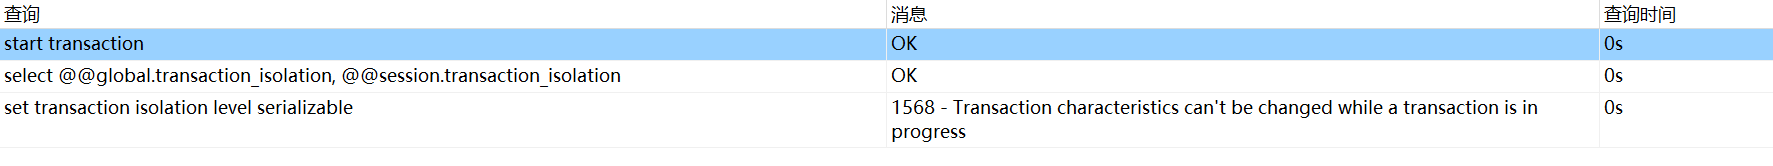
\includegraphics[width=0.9\textwidth]{img/44.png}
  \caption{T2 执行结果(4)}
\end{figure}

事务正在执行时,不能修改当前事务的隔离级别。

分别在不同客户端中执行下列语句,关注如何查询事务的状态;

\begin{lstlisting}[language=sql]
set innodb_lock_wait_timeout = 600; -- T1
set innodb_lock_wait_timeout = 600; -- T2
set innodb_lock_wait_timeout = 600; -- T3
set session transaction isolation level read committed; -- T1
start transaction; -- T1
set session transaction isolation level repeatable read; -- T2
start transaction; -- T2
set session transaction isolation level serializable;
start transaction; -- T3
select trx_id, trx_state, trx_isolation_level, trx_is_read_only from
information_schema.innodb_trx; -- T1
select * from performance_schema.processlist; -- T1
select * from performance_schema.data_locks; -- T1
select * from region; -- T1
select * from nation limit 5; -- T2
select * from customer limit 5; -- T3
select trx_id, trx_state, trx_isolation_level, trx_is_read_only from
information_schema.innodb_trx; -- T1
select * from performance_schema.processlist; -- T1
select engine_transaction_id, thread_id, object_schema, object_name,
lock_type, lock_mode, lock_data from performance_schema.data_locks; -- T1
insert into nation values(8888,'TEST',1,'It is a test.'); -- T1
update nation set n_comment = 'It is a test.' where n_nationkey = 0; -- T1
insert into customer
values(99999,'Nobody','Nowhere',10,'12345678',3.14,'BUILDING','It is a
test.'); -- T2
update customer set c_comment = 'It is a test.' where c_custkey = 1; -- T2
insert into region values(5,'MOON','It is a test.'); -- T3
update region set r_comment = 'It is a test.' where r_regionkey = 0; -- T3
select trx_id, trx_state, trx_isolation_level, trx_is_read_only from
information_schema.innodb_trx; -- T1
select * from performance_schema.processlist; -- T1
select engine_transaction_id, thread_id, object_schema, object_name,
lock_type, lock_mode, lock_data from performance_schema.data_locks; -- T1
SELECT r.trx_id waiting_trx_id, r.trx_mysql_thread_id waiting_thread,
r.trx_query waiting_query, b.trx_id blocking_trx_id, b.trx_mysql_thread_id
blocking_thread, b.trx_query blocking_query FROM
performance_schema.data_lock_waits w INNER JOIN
information_schema.innodb_trx b ON b.trx_id =
w.blocking_engine_transaction_id INNER JOIN information_schema.innodb_trx r
ON r.trx_id = w.requesting_engine_transaction_id; -- T1
SELECT waiting_trx_id, waiting_pid, waiting_query, blocking_trx_id,
blocking_pid, blocking_query FROM sys.innodb_lock_waits; -- T1
rollback; -- T3
rollback; -- T2
rollback; -- T1
\end{lstlisting}

结果如下:

\begin{figure}[H]
  \centering
  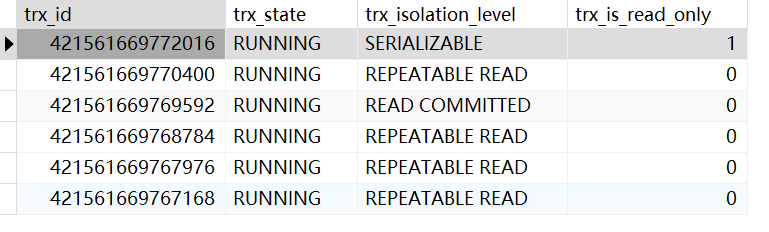
\includegraphics[width=0.9\textwidth]{img/45.png}
  \caption{执行结果(1)}
\end{figure}

\begin{figure}[H]
  \centering
  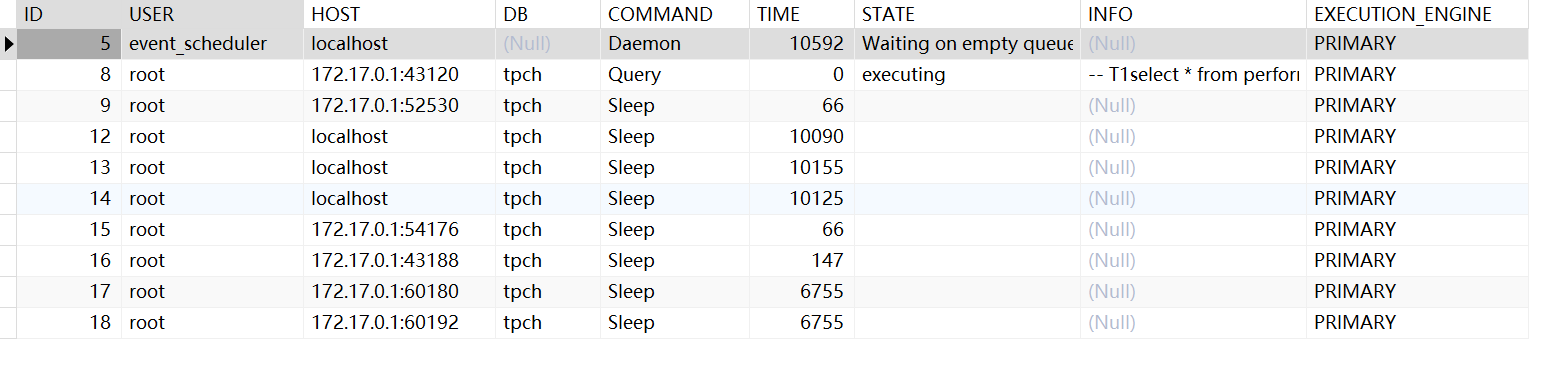
\includegraphics[width=0.9\textwidth]{img/46.png}
  \caption{执行结果(2)}
\end{figure}

\begin{figure}[H]
  \centering
  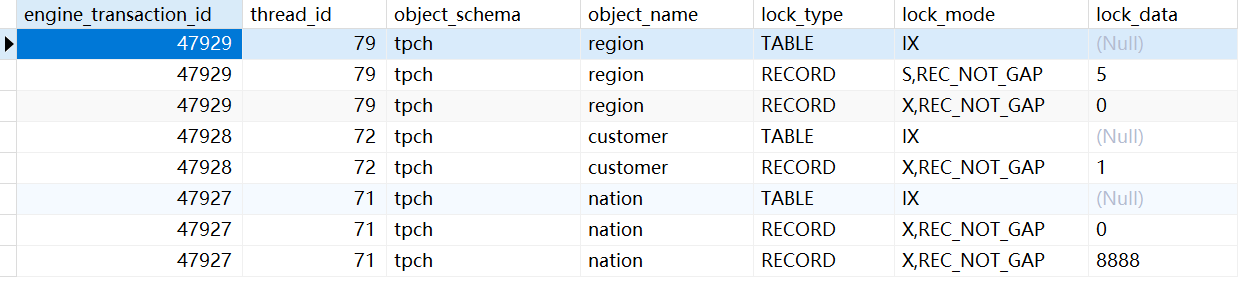
\includegraphics[width=0.9\textwidth]{img/47.png}
  \caption{执行结果(3)}
\end{figure}

\subsection{异常与隔离级别}

\subsubsection{Dirty Write}

\begin{lstlisting}[language=sql]
drop table if exists test_dirty_write;
create table test_dirty_write(id int primary key, value int) engine=innodb;
insert into test_dirty_write(id, value) values(1, 10), (2, 20);

set session transaction isolation level read uncommitted; begin; -- T1
set session transaction isolation level read uncommitted; begin; -- T2

update test_dirty_write set value = 11 where id = 1; -- T1
update test_dirty_write set value = 12 where id = 1; -- T2 (blocked here)

commit; -- T2 

commit; -- T1

select * from test_dirty_write; -- Shows 1 => 12, 2 => 20
\end{lstlisting}

在四种隔离级别下,均被阻塞在T2试图更改时,没有异常出现。

\subsubsection{Dirty Read}

\begin{lstlisting}[language=sql]
drop table if exists test_dirty_read;
create table test_dirty_read(id int primary key, value int) engine=innodb;
insert into test_dirty_read(id, value) values(1, 10), (2, 20);

set session transaction isolation level read uncommitted; begin; -- T1
set session transaction isolation level read uncommitted; begin; -- T2

-- T1更新数据,但不提交
update test_dirty_read set value = 11 where id = 1; -- T1

-- T2读取未提交的数据
select * from test_dirty_read; -- T2, Shows 1 => 11, 2 => 20

-- T1回滚更改
rollback; -- T1

-- T2再次读取数据
select * from test_dirty_read; -- T2, Shows 1 => 10, 2 => 20

commit; -- T2
\end{lstlisting}

只有在READ UNCOMMITTED隔离级别下,出现了脏读。

\begin{figure}[H]
\centering
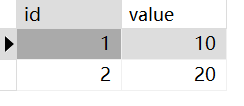
\includegraphics[width=0.3\textwidth]{img/48.png}
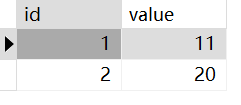
\includegraphics[width=0.3\textwidth]{img/49.png}
\caption{READ UNCOMMITTED隔离级别下的脏读}
\end{figure}

\begin{figure}[H]
\centering
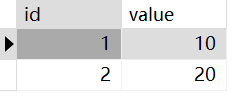
\includegraphics[width=0.3\textwidth]{img/50.png}
\includegraphics[width=0.3\textwidth]{img/51.png}
\caption{其他隔离级别下无异常}
\end{figure}

\subsubsection{Non-Repeatable Read}

\begin{lstlisting}[language=sql]
drop table if exists test_non_repeatable_read;
create table test_non_repeatable_read(id int primary key, value int) engine=innodb;
insert into test_non_repeatable_read(id, value) values(1, 10), (2, 20);

set session transaction isolation level read uncommitted; begin; -- T1
set session transaction isolation level read uncommitted; begin; -- T2

-- T1读取数据
select * from test_non_repeatable_read; -- T1, Shows 1 => 10, 2 => 20

-- T2更新数据并提交
update test_non_repeatable_read set value = 11 where id = 1; -- T2
commit; -- T2

-- T1再次读取同一行的数据
select * from test_non_repeatable_read where id = 1; -- T1, Shows 1 => 11

commit; -- T1
\end{lstlisting}

READ UNCOMMITTED隔离级别和READ COMMITTED隔离级别下,出现了不可重复读。

\begin{figure}[H]
\centering
\includegraphics[width=0.3\textwidth]{img/52.png}
\includegraphics[width=0.3\textwidth]{img/53.png}
\caption{READ UNCOMMITTED 和 READ COMMITTED 隔离级别下的不可重复读}
\end{figure}

\begin{figure}[H]
\centering
\includegraphics[width=0.3\textwidth]{img/54.png}
\includegraphics[width=0.3\textwidth]{img/55.png}
\caption{其他隔离级别下无异常}
\end{figure}

\subsubsection{Phantom Read}

\begin{lstlisting}[language=sql]
drop table if exists test_phantom_read;
create table test_phantom_read(id int primary key, value int) engine=innodb;
insert into test_phantom_read(id, value) values(1, 10), (2, 20);

set session transaction isolation level read committed; begin; -- T1
set session transaction isolation level read committed; begin; -- T2

-- T1读取数据
select * from test_phantom_read; -- T1, Shows 1 => 10, 2 => 20

-- T2插入新数据并提交
insert into test_phantom_read(id, value) values(3, 30); -- T2
commit; -- T2

-- T1再次读取数据,发现多了一行新的数据
select * from test_phantom_read; -- T1, Shows 1 => 10, 2 => 20, 3 => 30

commit; -- T1
\end{lstlisting}

除了SERIALIZABLE隔离级别外,其他隔离级别下,出现了幻读。

\begin{figure}[H]
\centering
\includegraphics[width=0.3\textwidth]{img/56.png}
\includegraphics[width=0.3\textwidth]{img/57.png}
\caption{READ UNCOMMITTED, READ COMMITTED 和 REPEATABLE READ 隔离级别下的幻读}
\end{figure}

\subsubsection{Lost Update}

\begin{lstlisting}[language=sql]
drop table if exists test_lost_update;
create table test_lost_update(id int primary key, value int) engine=innodb;
insert into test_lost_update(id, value) values(1, 10), (2, 20);

set session transaction isolation level REPEATABLE READ; begin; -- T1
set session transaction isolation level REPEATABLE READ; begin; -- T2

-- T1读取数据
select value from test_lost_update where id = 1; -- T1, Shows 10

-- T2读取数据
select value from test_lost_update where id = 1; -- T2, Shows 10

-- T1更新数据
update test_lost_update set value = 11 where id = 1; -- T1

-- T2更新数据
update test_lost_update set value = 12 where id = 1; -- T2

-- 提交T1
commit; -- T1

-- 提交T2
commit; -- T2

-- 检查表中的数据
select * from test_lost_update; -- Shows 1 => 12, 2 => 20
\end{lstlisting}

除了 SERIALIZABLE 隔离级别外,其他隔离级别下,均在 T2 更新数据时,被阻塞。
而 SERIALIZABLE 隔离级别下,T1 更新数据时就发生阻塞,T2 更新数据时,报出了死锁异常。

\begin{figure}[H]
\centering
\includegraphics[width=\textwidth]{img/59.png}
\caption{死锁异常}
\end{figure}

\subsubsection{Read Skew}

\begin{lstlisting}[language=sql]
drop table if exists test_read_skew;
create table test_read_skew(id int primary key, value int) engine=innodb;
insert into test_read_skew(id, value) values(1, 10), (2, 20);

set session transaction isolation level REPEATABLE READ; begin; -- T1
set session transaction isolation level REPEATABLE READ; begin; -- T2

-- T1读取数据
select * from test_read_skew where id = 1; -- T1, Shows 1 => 10

-- T2更新数据并提交
update test_read_skew set value = 11 where id = 1; -- T2
commit; -- T2

-- T1再次读取同一行的数据
select * from test_read_skew where id = 1; -- T1, Shows 1 => 11

commit; -- T1
\end{lstlisting}

READ UNCOMMITTED隔离级别和READ COMMITTED隔离级别下,出现了读偏斜。

\begin{figure}[H]
\centering
\includegraphics[width=0.3\textwidth]{img/60.png}
\includegraphics[width=0.3\textwidth]{img/61.png}
\caption{READ UNCOMMITTED 和 READ COMMITTED 隔离级别下的读偏斜}
\end{figure}

\begin{figure}[H]
\centering
\includegraphics[width=0.3\textwidth]{img/62.png}
\includegraphics[width=0.3\textwidth]{img/63.png}
\caption{其他隔离级别下无异常}
\end{figure}

\subsubsection{Write Skew}

\begin{lstlisting}[language=sql]
drop table if exists test_write_skew;
create table test_write_skew(id int primary key, value int) engine=innodb;
insert into test_write_skew(id, value) values(1, 10), (2, 20);

set session transaction isolation level REPEATABLE READ; begin; -- T1
set session transaction isolation level REPEATABLE READ; begin; -- T2

select * from test_write_skew where id in (1, 2); -- T1, Shows 1 => 10, 2 => 20
select * from test_write_skew where id in (1, 2); -- T2, Shows 1 => 10, 2 => 20

update test_write_skew set value = 11 where id = 1; -- T1
update test_write_skew set value = 21 where id = 1; -- T2

commit; -- T1
commit; -- T2
\end{lstlisting}

除 SERIALIZABLE 隔离级别外,其他隔离级别下,均在 T2 更新数据时,被阻塞。
而 SERIALIZABLE 隔离级别下,T1 更新数据时就发生阻塞,T2 更新数据时,报出了死锁异常。

\begin{figure}[H]
\centering
\includegraphics[width=\textwidth]{img/64.png}
\caption{死锁异常}
\end{figure}
\begin{table}[h!]
  \centering
  \resizebox{\textwidth}{!}{
  \begin{tabular}{|c|c|c|c|c|c|}
      \hline
      \textbf{Anomalies/Isolation Level} & \textbf{READ UNCOMMITTED} & \textbf{READ COMMITTED} & \textbf{REPEATABLE READ} & \textbf{SERIALIZABLE} \\
      \hline
      Dirty Write & \checkmark & \checkmark & \checkmark & \checkmark \\
      \hline
      Dirty Read & $\times$ & \checkmark & \checkmark & \checkmark \\
      \hline
      Non-repeatable Read & $\times$ & $\times$ & \checkmark & \checkmark \\
      \hline
      Phantom Read & $\times$ & $\times$ & $\times$ & \checkmark \\
      \hline
      Lost Update & $\times$ & $\times$ & $\times$ & \checkmark \\
      \hline
      Read Skew & $\times$ & $\times$ & \checkmark & \checkmark \\
      \hline
      Write Skew & $\times$ & $\times$ & $\times$ & \checkmark \\
      \hline
  \end{tabular}
  }
  \caption{Isolation Levels and Anomalies}
  \label{table:isolation_anomalies}
\end{table}


\section{存在的问题及解决方案}

\begin{enumerate}
  \item 显示当前为只读事务时,无法插入数据;
  
  解决方案:在事务开始前设置事务为读写事务。
\end{enumerate}


\section{实验小结}

通过本次实验,我学习了MySQL数据库管理系统中事务处理相关的设置和基本操作,以及事务处理过程中不同事务隔离级别所对应的异常,能够根据应用场景选择合适的事务隔离级别。


\end{document}